\chapter{Paketeinteilung}
\label{ch:paketeinteilung}

Die Paketeinteilung der Software gliedert sich in folgende Pakete: %TODO Paketübersicht

\section{graphmodel}

\begin{figure}[hb]
  \centering
  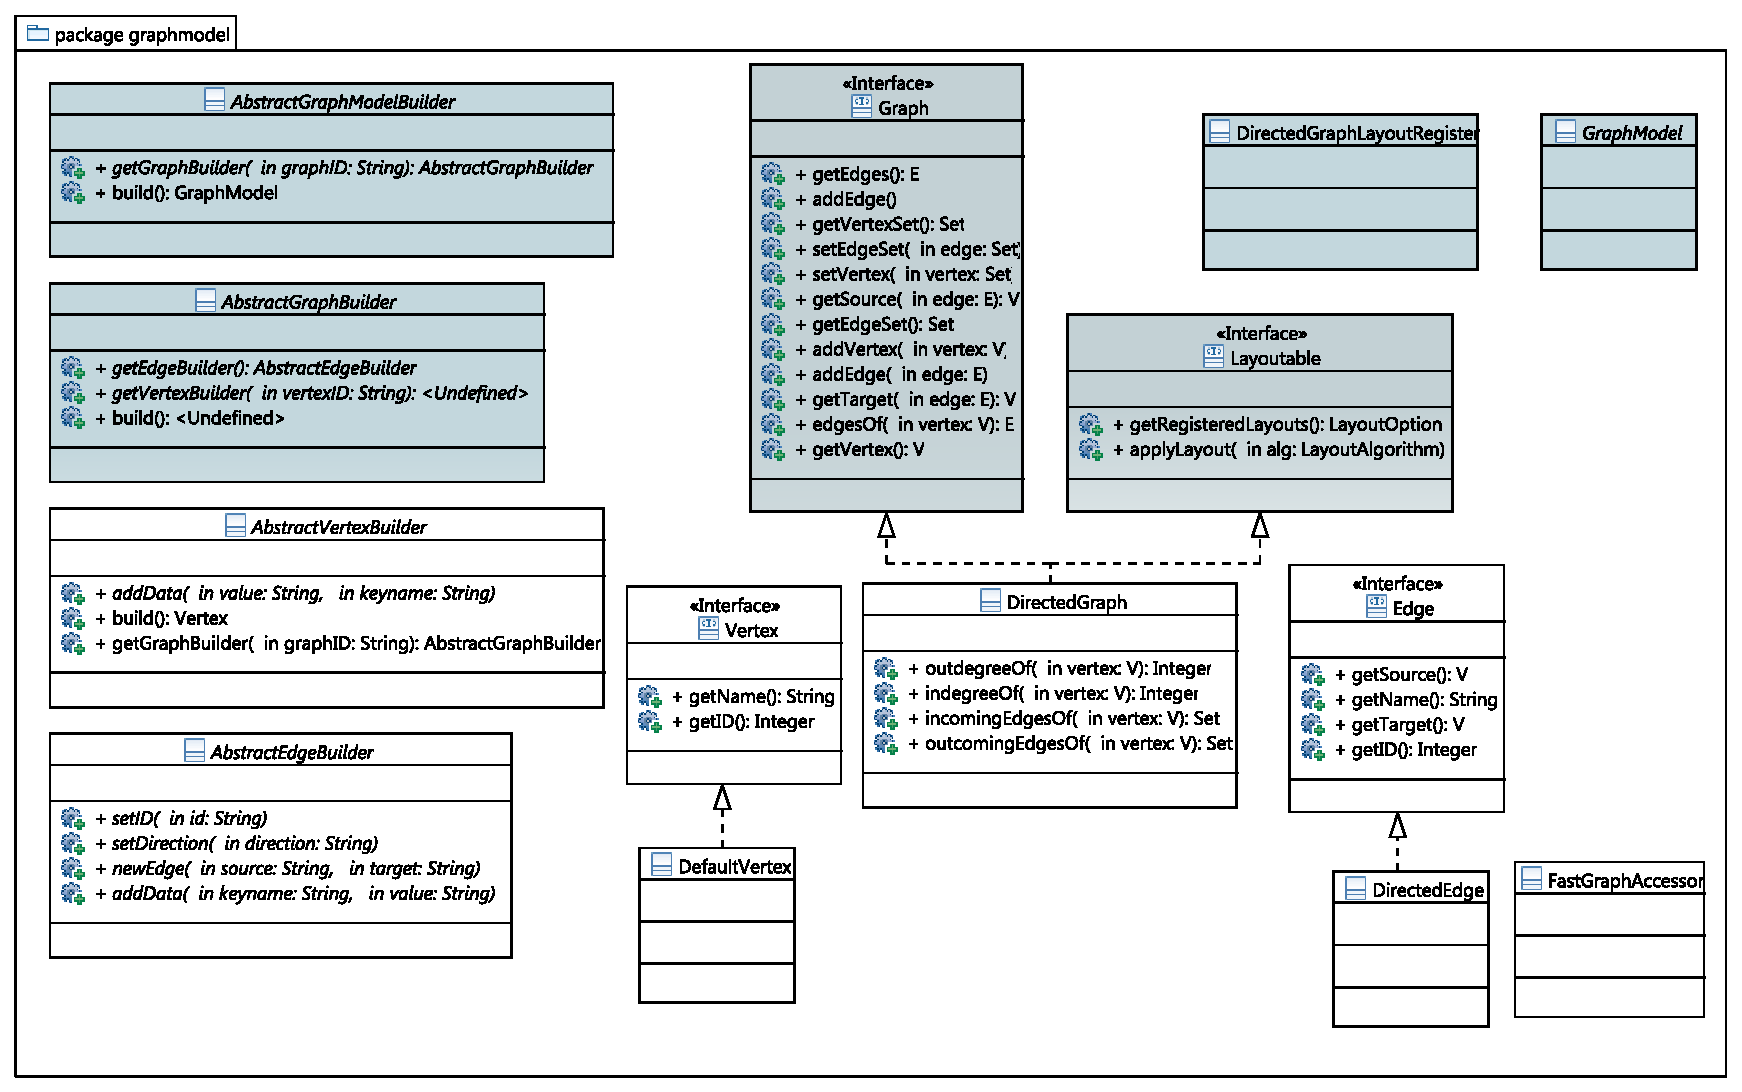
\includegraphics[width=380pt]{resourcen/graphmodel.pdf}
  \caption{Paketübersicht graphmodel}
  \label{fig:packge_graphmodel}
\end{figure}

In dem Paket graphmodel befinden sich die Klassen die für die interne Repräsentation des Graphen benötigt werden. Die Funktionalität dieses Pakets ist es ein flexibles Graph-Modell, sowie schnellen Zugriff auf dessen Komponenten bereitzustellen.\\ 
Zum Graph-Modell gehören Interfaces wie GraphModel, Graph, Vertex und Edge welche den groben Aufbau eines Graphen und dessen Funktionalitäten vorgeben. Das GraphModel enthält alle Graphen, welche bei einem Import aus der Datei ausgelesen wurden. Da es Kanten und somit auch Graphen gibt, welche gerichtet sind, gibt es dazu auch passende Interfaces, welche die zuvor genannten erweitern. Zusätzlich gibt es noch weitere Spezialisierungen der Interfaces, wie CompoundVertex, ein Knoten der einen Subgraphen enthält und LayeredGraph, ein Graph der noch Schichten speichert.\\
Die genannten Interfaces sind teilweise schon implementiert. Zu diesen Klassen gehören die Default-Klassen, welche die im Interface definierten Methoden primitiv implementieren und die Serialized-Klassen, welche ein jeweiliges Element darstellt, welches einheitlich für den Export vorbereitet ist. \\
Damit speziellere Implementierungen von Graph, Vertex oder Edge aus Plugins vom Importer einheitlich erstellt werden können gibt es die Builder-Interfaces. Sie geben eine Schnittstelle vor, über welche die speziellen Graphelemente erstellt werden können, ohne das der Importer davon etwas wissen muss.

\newpage

\section{gui}

\begin{figure}[hb]
  \centering
  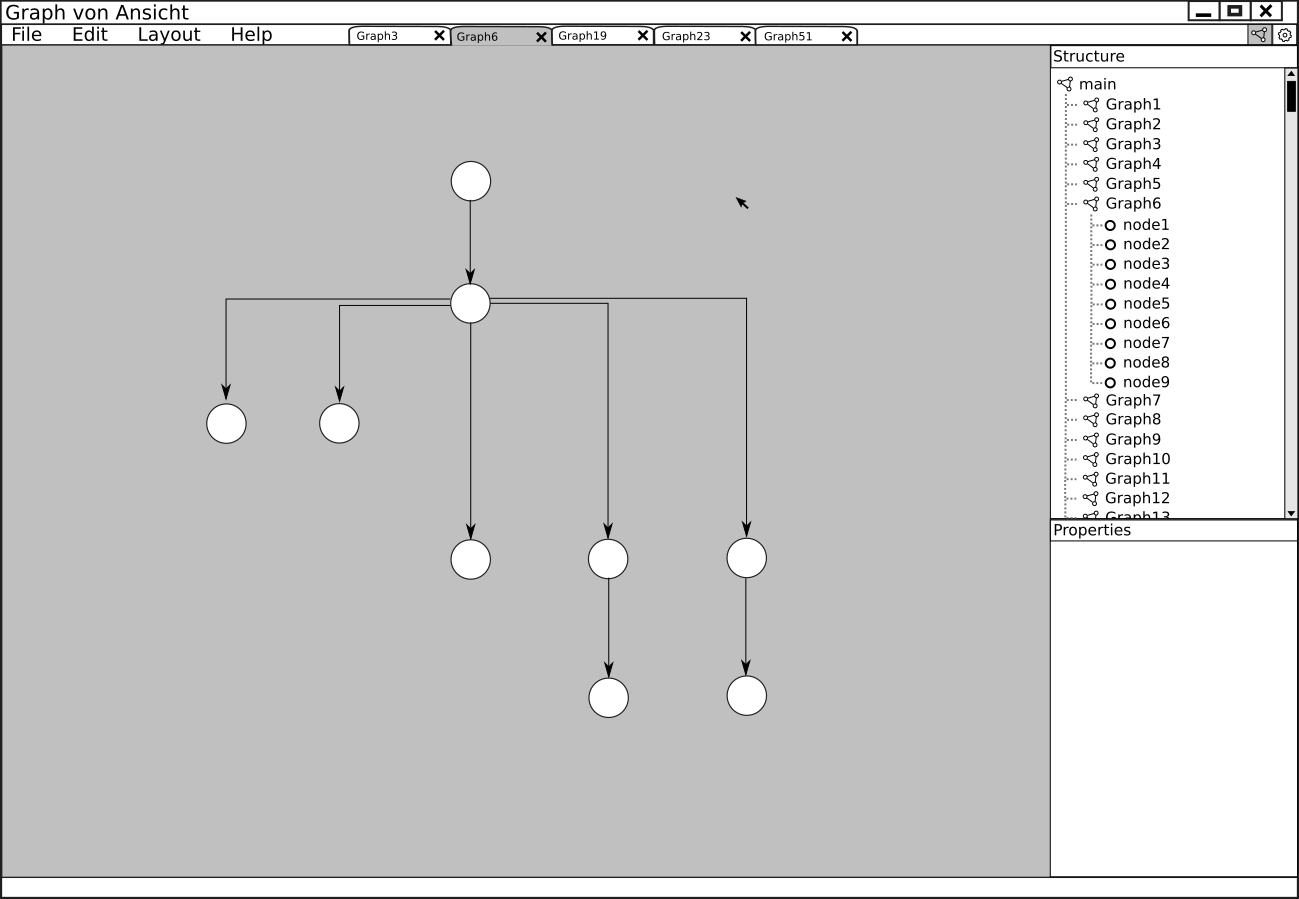
\includegraphics[width=380pt]{resourcen/gui.pdf}
  \caption{Paketübersicht gui}
  \label{fig:packge_gui}
\end{figure}

Das Paket \textbf{gui} beinhaltet die Anzeigelogik, sowie die Haupt-Applikation von GAns. Dafür werden JavaFX Komponenten verwendet, die erweitert und angepasst werden. Es werden Views und Elemente definiert, die für die Anzeige notwendig sind. Die \textbf{GAnsApplication} hat, als Klasse welche das ganze Programm aufsetzt, noch weitere Aufgaben. Sie stößt das Laden der Plugins an und behandelt zusätzlich viele Interaktionen des Benutzers mit den einzelnen GUI-Elementen(siehe SeqDiag Import, doppelklick, selection) unter anderem auch das Laden bzw. Erstellen des unterliegenden GraphModels(siehe graphmodel). Es werden verschiedene Views definiert:
\begin{enumerate}
	\item[\textbf{GraphView}] Eine View welche den gelayouteten Graphen anzeigt und dazu verschiedene Navigationsmöglichkeiten, wie Zoom, Selektion usw., anbietet. Es können mehrere GraphViews gleichzeitig geöffnet sein. Jede einzelne ist in einem eigenen Tab enthalten, zwischen denen hin und her gewechselt werden kann. Die Elemente welche in der GraphView angezeigt werden, sind \textbf{GAnsGraphElemente}. Sie bestehen aus verschiedenen JavaFX Klassen, welche einen Text und eine Farbe gesetzt bekommen können. Standardmäßig werden Rechtecke für Knoten und direkte Kanten als Kanten zwischen Knoten verwendet.
	\item[\textbf{StructureView}] Eine TreeView, welche die geschachtelten Graphen einer importierten Datei anzeigt. Über doppelklick auf eines der Baumelemente wird der durch das Element dargestellte Graph in einer neuen GraphView angezeigt. Zum Erstellen der einzelnen Baumelemente werden normale JavaFX-Funktionalitäten verwendet.
	\item[\textbf{InformationView}] Eine TableView, welche, je nach Selektion in der aktuell angezeigten GraphView, Informationen über die selektierten Elemente anzeigt. Jede Zeile der Tabelle enthält in der ersten Zelle den Bezeichner/Namen und in der zweiten Zelle den jeweiligen Wert der Eigenschaft aus der Selektion. Die einzelnen Zellen werden durch eine JavaFX \textbf{PropertyValueFactory} erstellt welche mit den \textbf{GAnsProperties}(siehe objectproperty) der selektierten Elemente der GraphView arbeitet.
\end{enumerate}}

\newpage

\section{parameter}

\begin{figure}[hb]
  \centering
  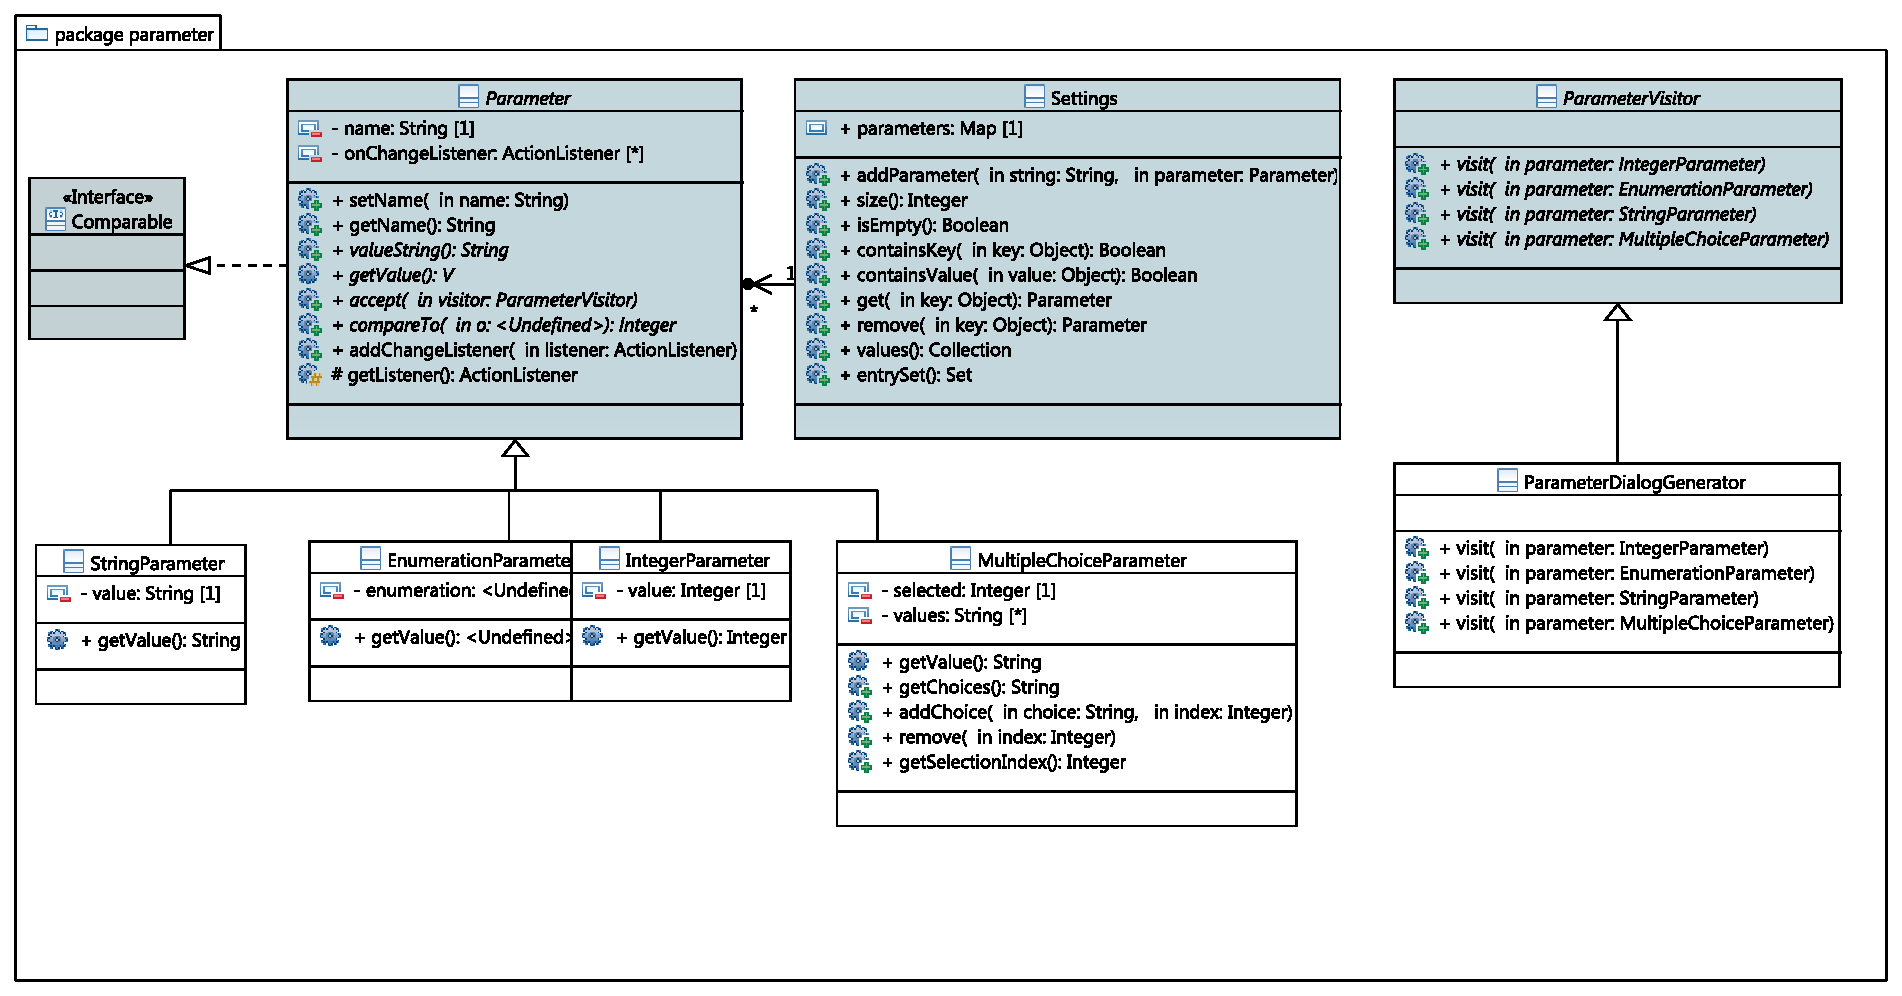
\includegraphics[width=380pt]{resourcen/parameter.pdf}
  \caption{Paketübersicht parameter}
  \label{fig:packge_parameter}
\end{figure}

Diese Paket trennt parameter vom Rest. Diese speziellen Wrapper erlauben dem plugins ihre Einstellungen an den View zu übergeben. Das selbe gilt auch für Constraints. Diese Wrapper Klassen beinhalten Methoden zur Umwandlung der jeweiligen Parameter in Zeichenketten aber auch vergleiche zum sortieren der Werte.

\newpage

\section{graphRegex}

\begin{figure}[hb]
  \centering
  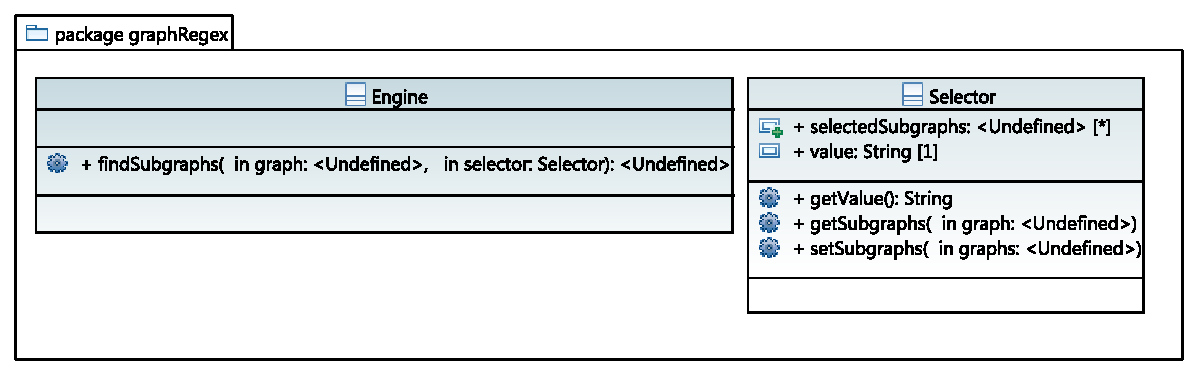
\includegraphics[width=380pt]{resourcen/graphRegex.pdf}
  \caption{Paketübersicht graphRegex}
  \label{fig:packge_graphRegex}
\end{figure}

In diesem Paket befinden sich die Algorithmen zum durchsuchen von Graphen nach Subgraphen mithilfe von Selektoren

\newpage

\section{objectproperty}

\begin{figure}[hb]
  \centering
  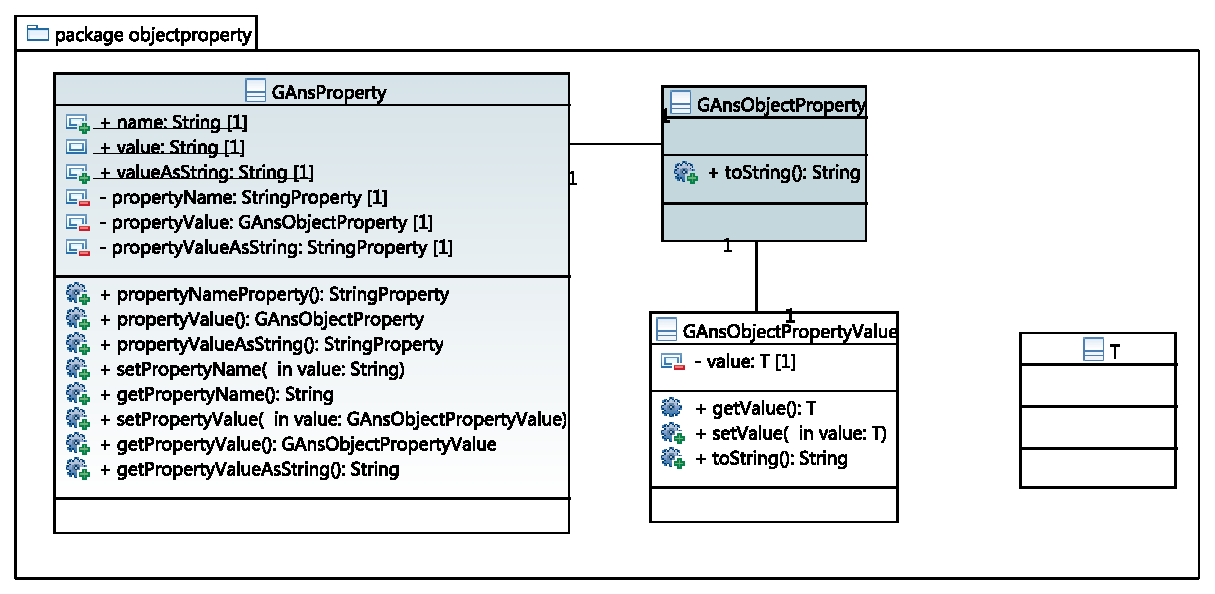
\includegraphics[width=380pt]{resourcen/objectproperty.pdf}
  \caption{Paketübersicht objectproperty}
  \label{fig:packge_objectproperty}
\end{figure}

Das Paket \textbf{objectproperty} bietet eine generische Eigenschaft eines Elements aus dem Paket \textbf{graphmodel}. Dabei stellt jede \textbf{GAnsProperty} eine einzelne Eigenschaft dar, welche aus einen Bezeichner/Namen, einen generischen Wert und eine Stringrepräsentation des Werts besteht. Die einzelnen Bestandteile werden in JavaFX ObjectProperties gespeichert. Darunter die \textbf{GAnsObjectProperty}, welche einen generischen Typ unterstützt. Diese Properties harmonieren gut mit den restlichen JavaFX-GUI-Elementen, somit kann auf viele Funktionen zurückgegriffen werden kann die von JavaFX direkt angeboten werden ohne große Eigenentwicklungen anfertigen zu müssen. Das beste Beispiel dafür ist die InformationView der GUI, deren Inhalt durch \textbf{PropertyValueFactories} von JavaFX automatisch erstellt werden, sobald eine Liste mit GAnsProperties gesetzt wird. Dabei ist der eigentliche Typ des Werts irrelevant, da in der GUI auf die Stringrepräsentation des Werts zugegriffen werden kann, wobei z.B. im Model oder Layoutalgorithmus mit dem eigentlichen Wert gearbeitet werden kann. Die PropertyValueFactories arbeiten mit dem Bestandteil der GAnsProperty, welcher mit einem bestimmten Referenz-String erstellt wurde. Diese Strings sind in GAnsProperty statisch gegeben, sodass die Aufrufe selbst bei Änderungen in der GAnsProperty im restlichen Programm konstant bleiben.

\newpage

\section{plugin}

\begin{figure}[hb]
  \centering
  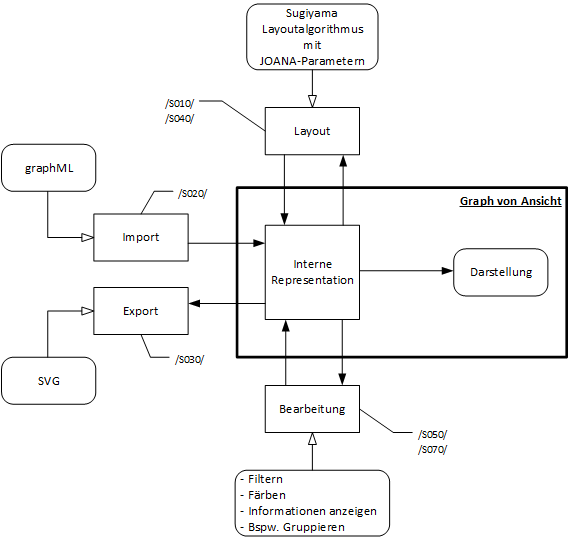
\includegraphics[width=380pt]{resourcen/plugin.pdf}
  \caption{Paketübersicht plugin}
  \label{fig:packge_plugin}
\end{figure}

\newpage

\section{sugiyama}

\begin{figure}[hb]
  \centering
  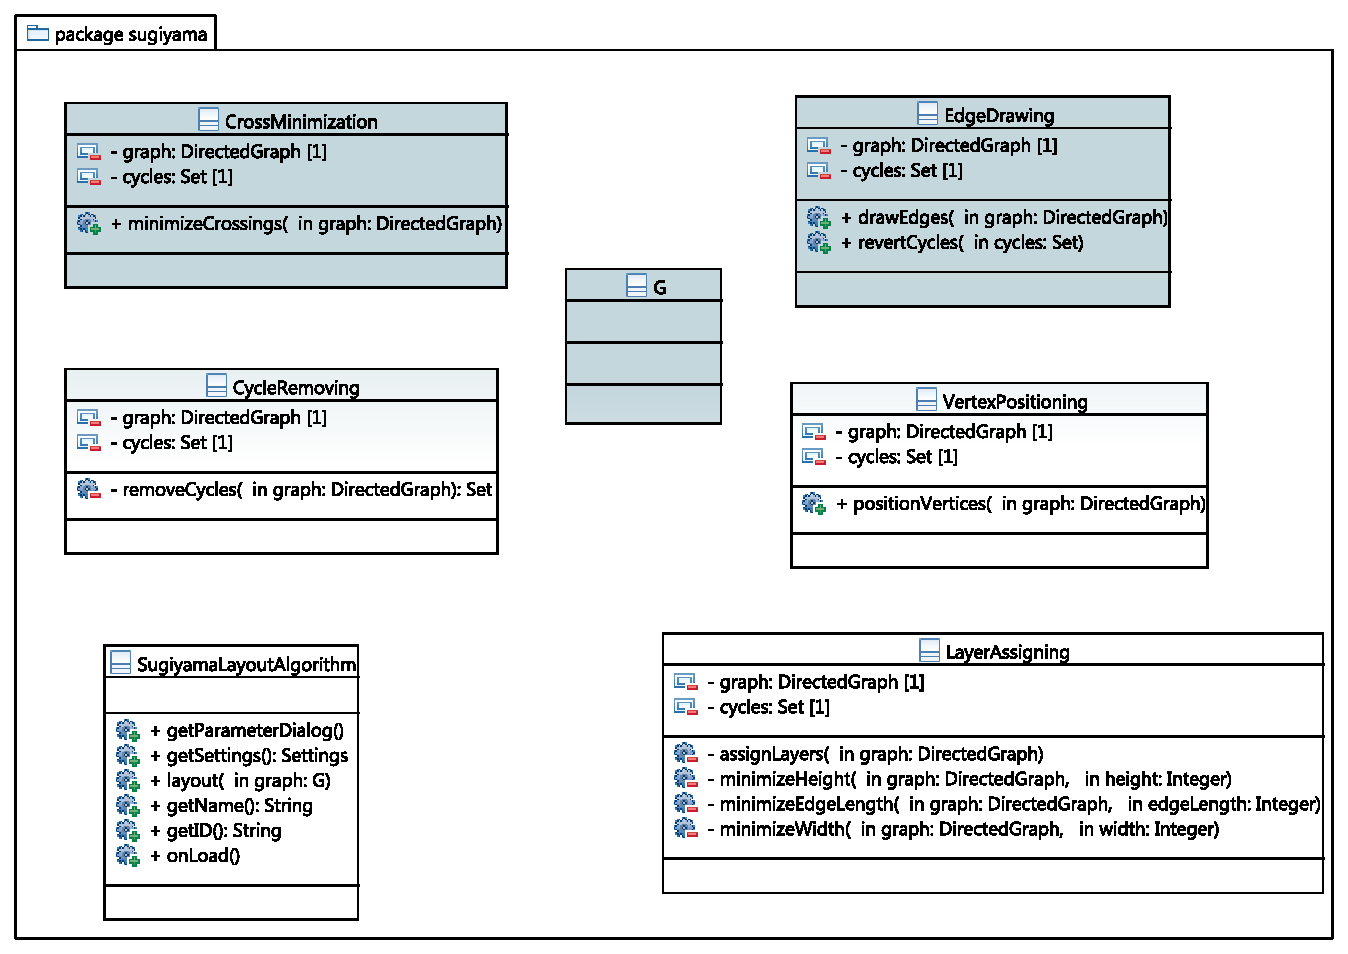
\includegraphics[width=380pt]{resourcen/sugiyama.pdf}
  \caption{Paketübersicht sugiyama}
  \label{fig:packge_sugiyama}
\end{figure}

Das Paket \textbf{sugiyama} bietet neben einer Implementierung des Sugiyama-Frameworks zum hierarchischen layouten eines gerichteten Graphen Schnittstellen zum ändern und austauschen einzelner Schritte dieses Frameworks.\\
Die fünf Schritte des Sugiyama-Frameworks Kreise entfernen, Lagenzuordnung, Kreuzungsminimierung, Knotenpositionierung und Kantenzeichnen werden in dieser Reihenfolge durchlaufen und durch einen \textbf{SugiyamaLayoutAlgorithm} verwaltet und gesteuert. Die Klassen, die diese Schritte darstellen \textbf{CycleRemover}, \textbf{LayerAssigner}, \textbf{CrossMinimizer}, \textbf{VertexPositioner} und \textbf{EdgeDrawer} arbeiten auf einem \textbf{SugiyamaGraph}, welcher den zu layoutenden Graphen repräsentiert.\\
Im ersten Schritt werden die Zykel des Graphen entfernt, indem die Richtungen einer minimalen Kantenmenge umgekehrt wird.\\
Anschließend wird jedem Knoten eine Lage zugewiesen, welche abhängig von der Anzahl der ein- und ausgehenden Kanten des Knotens, sowie der Länge des kürzesten Pfades des Knotens zu einem Knoten aus der ersten Lage ist. Zudem werden, falls eine Kante zwischen zwei Knoten mindestens eine Lage überspringt, in jede dieser Lagen ein \textbf{DummyVertex} ein.\\
Im dritten Schritt wird die Anzahl der Kantenkreuzungen minimiert. Dazu werden jeweils in zwei aneinanderliegenden Lagen die Knoten beider Lagen umgeordnet.\\
In Schritt Vier bekommen die Knoten feste Positionen in den Lagen zugewiesen\\
Im letzten Schritt wird jeder \textbf{DummyVertex} entfernt und die Kanten werden gezeichnet. Zusätzlich werden die im ersten Schritt umgedrehten Kanten wieder in ihre ursprüngliche Richtung zurückversetzt.

\newpage

\section{joana}

\begin{figure}[hb]
  \centering
  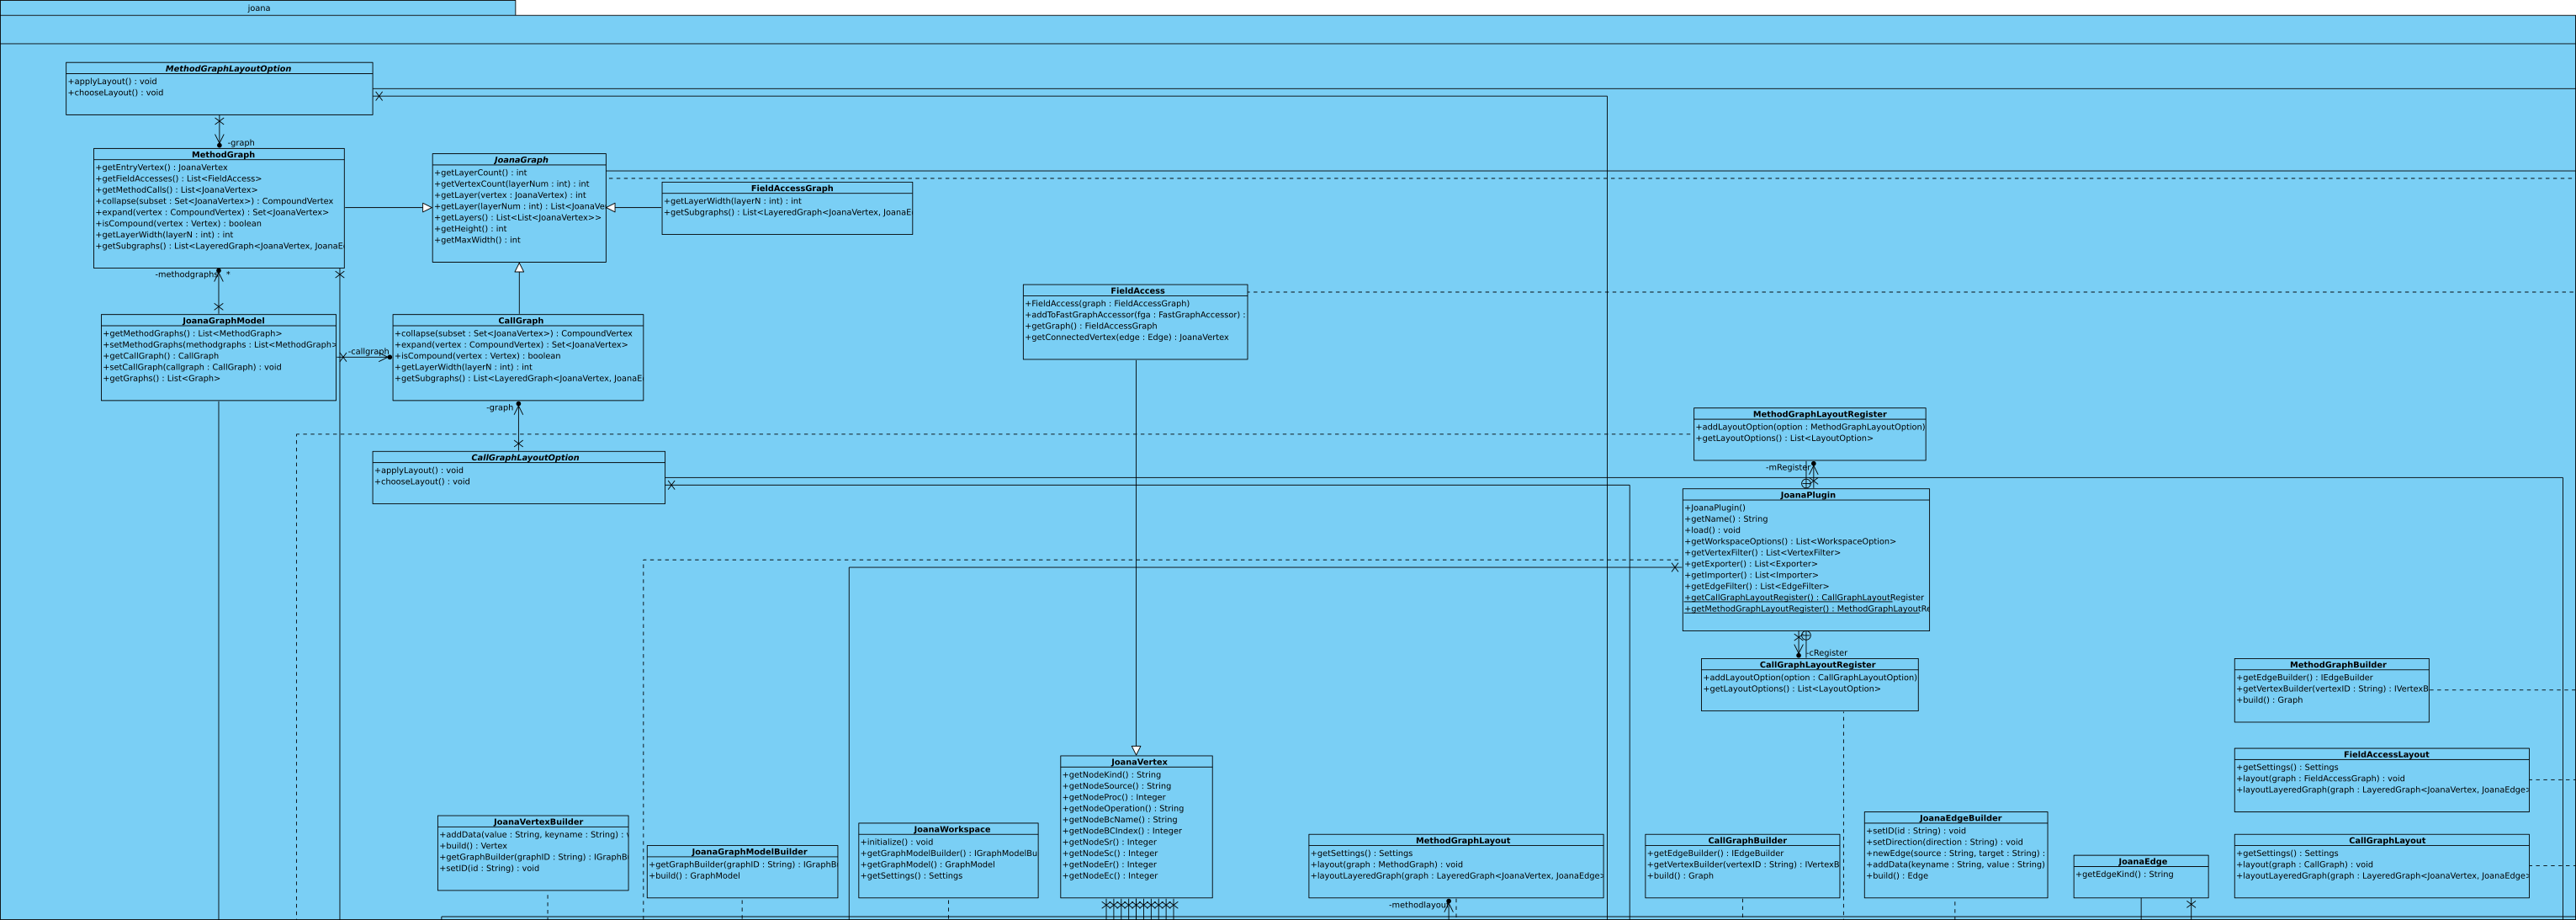
\includegraphics[width=380pt]{resourcen/joana.pdf}
  \caption{Paketübersicht joana}
  \label{fig:packge_joana}
\end{figure}

Das Paket Joana stellt ein weiteres mitgeliefertes Plugin dar und erweitert den sugiyama Algorithmus um spezifische Einstellungen und Constraints für Joana Graphen. Zu dem stellt es die Graphtypen Methoden- und Callgraph bereit, welche Joana spezifisch sind.